\documentclass[aspectratio=43, dvipsnames]{beamer}
\usepackage[version=4]{mhchem}
\usepackage[aboveskip=1pt, belowskip=1pt]{caption}
\usepackage{amsmath}
\usepackage{siunitx}
\usepackage{emoji}
\usepackage{pgfplots}
\pgfplotsset{compat=1.18,}

% Command to display isotopes
\newcommand{\iso}[2]{\ce{^{#1}#2}}
% Command to write overlap
\newcommand{\overlap}[2]{\left\langle#1\middle\vert#2\right\rangle}
% Command to write Rs
\newcommand{\rs}{$\text{R}_{\text{S}}$ }
% Command to draw enumitems outside the environment
\newcommand{\enumitem}[1]{%
\setcounter{enumi}{#1}\usebeamertemplate{enumerate item}% 
}
\newcommand{\boxitem}[1]{\raisebox{0.15em}{\enumitem{#1}}}
% Set caption package options
\captionsetup{labelformat=empty, font={rm,footnotesize}}

\title[Oxygen spectroscopy]{Low-lying spectroscopy of \iso{19,20}{O}}
\date[March 2025]{March 2025}
\author[M. Lozano et al.]{M. Lozano-González, B. Fernández-Domínguez, \texorpdfstring{\newline}{} J. Lois-Fuentes, F. Delaunay}
\institute{USC-IGFAE and LPC-Caen}

\usetheme{igfae}

\begin{document}

\maketitle

\section{Experimental setup}
\begin{frame}{Experimental setup}
	E796 was performed at LISE (GANIL) back in March 2022 under these experimental conditions:
	\begin{columns}[t]
		\begin{column}{0.5\linewidth}
			\begin{itemize}
				\item Beam: \iso{20}{O} @ \qty{35}{A\MeV}
				\item Gas: \qty{90}{\percent}\ce{D_2} and \qty{10}{\percent} \ce{iC_4H_{10}}
				\item Silicons: two front layers and one left. \qty{500}{\micro\m}-thick
			\end{itemize}
			\begin{columns}[c]
				\begin{column}{0.5\linewidth}
					\mycolorbox[1]{boxPink}{
						\textbf{(In)elastic}\\
						$\iso{20}{O}(\iso{}{p}, \iso{}{p})$\\
						$\iso{20}{O}(\iso{}{d}, \iso{}{d})$
					}\hfill
				\end{column}%
				\begin{column}{0.5\linewidth}
					\mycolorbox[1]{boxBrown}{
						\textbf{p and n removal}\\
						$\iso{20}{O}(\iso{}{d},\iso{3}{He})$\\
						$\iso{20}{O}(\iso{}{d},\iso{}{t})$\\
						$\iso{20}{O}(\iso{}{p},\iso{}{d})$\\
					}
				\end{column}
			\end{columns}
		\end{column}\hfil
		\begin{column}{0.45\linewidth}
			\begin{figure}
				\begin{center}
					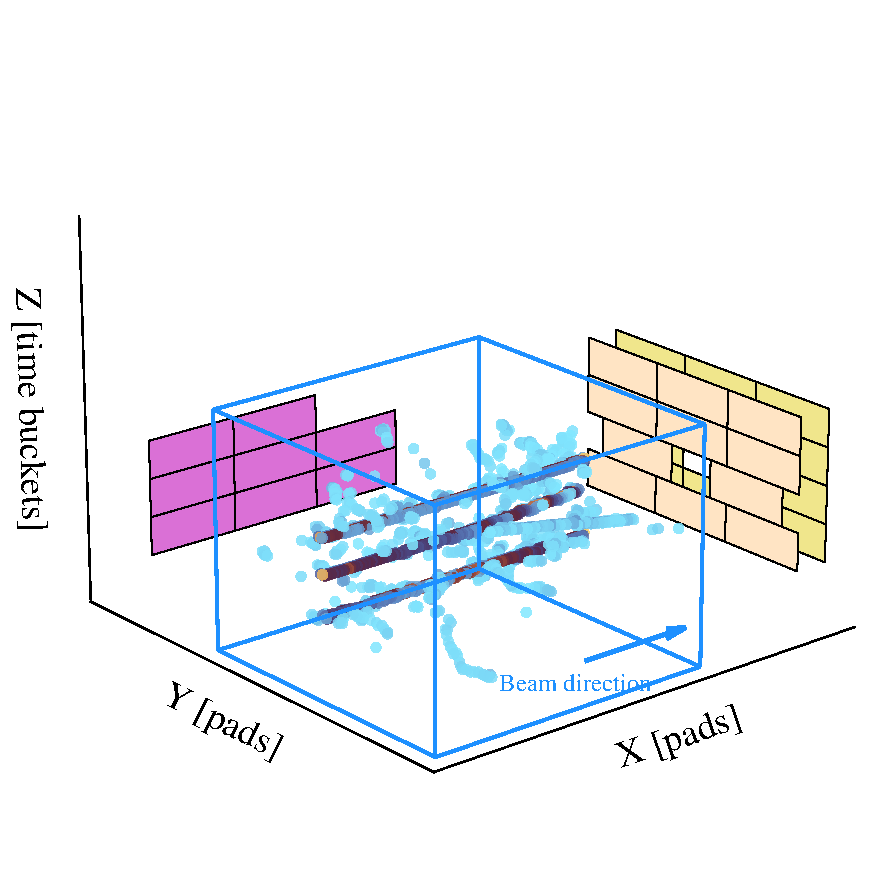
\includegraphics[width=0.95\textwidth]{figures/setup.pdf}
				\end{center}
			\end{figure}

		\end{column}
	\end{columns}

\end{frame}

\section{Motivation}
% \begin{frame}[c]{Physics case}
% 	\textbf{Inelastic}: \iso{20}{O}(p,p') and (d,d') excitations
% 	\bigskip
% 	\begin{columns}[c]
% 		\begin{column}{0.5\linewidth}
% 			\mycolorbox{boxBrown}{
% 				Probing their \textbf{isoscalar} or \textbf{isovector} character
% 				\begin{enumerate}
% 					\item Determine $\beta_{nucl}$ from xs normalization
% 					\item Use previous $B(E2)$
% 					\item Bernstein formula for $M_{n}/M_{p}$ ratio
% 				\end{enumerate}
% 			}
% 		\end{column}%
% 		\begin{column}{0.5\linewidth}
% 			\mycolorbox[1]{boxGreen}{
% 				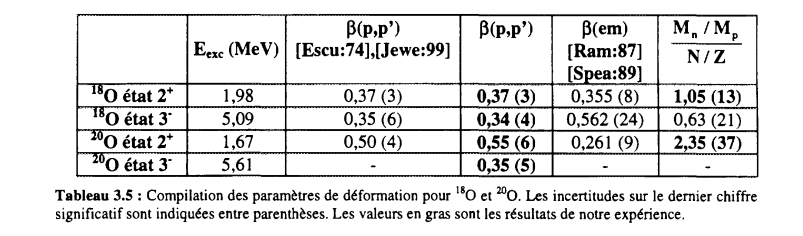
\includegraphics[width=1\linewidth]{figures/khan.png}
% 				{\small\itshape E.Khan thesis (2000)}
% 				\begin{itemize}
% 					\item $\sim 1 \Rightarrow$ isoscalar
% 					\item $\gg 1 \Rightarrow$ isovector
% 				\end{itemize}
% 			}
% 		\end{column}
% 	\end{columns}
% \end{frame}

\begin{frame}[c]{Physics case}
	\textbf{Transfer}: spectroscopy on \iso{20}{O}(d,t),(p,d)\iso{19}{O}
	\begin{equation*}
		\left.\frac{d\sigma}{d\Omega}\right\vert_{\text{exp}} = C^{2}S \cdot \left.\frac{d\sigma}{d\Omega}\right\vert_{\text{s.p}}, \quad \sum C^{2}S = (2j + 1)
	\end{equation*}
	\bigskip
	\begin{columns}[c]
		\begin{column}{0.5\linewidth}
			\mycolorbox{boxBrown}{
				Two goals:
				\begin{enumerate}
					\item Study of the \iso{20}{O} gs wave-function
					\item Behaviour of $\mathcal{N} = 8$ gap
				\end{enumerate}
			}
		\end{column}%
		\begin{column}{0.5\linewidth}
			\mycolorbox[1]{boxGreen}{
				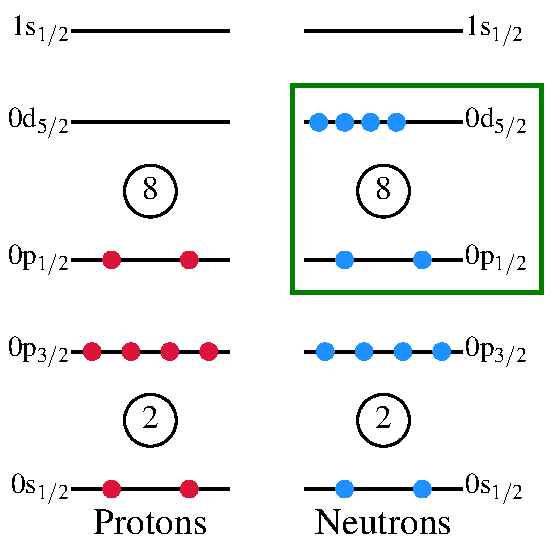
\includegraphics[width=0.7\linewidth]{figures/sm.pdf}
				\captionof{figure}{\iso{20}{O} shell-model prediction}
			}
		\end{column}
	\end{columns}
\end{frame}

\section{Analysis}
\begin{frame}{A glance at the analysis}
	Independent analyis from Juan: same general idea but different execution and (I hope) some improvements.
	\begin{figure}
		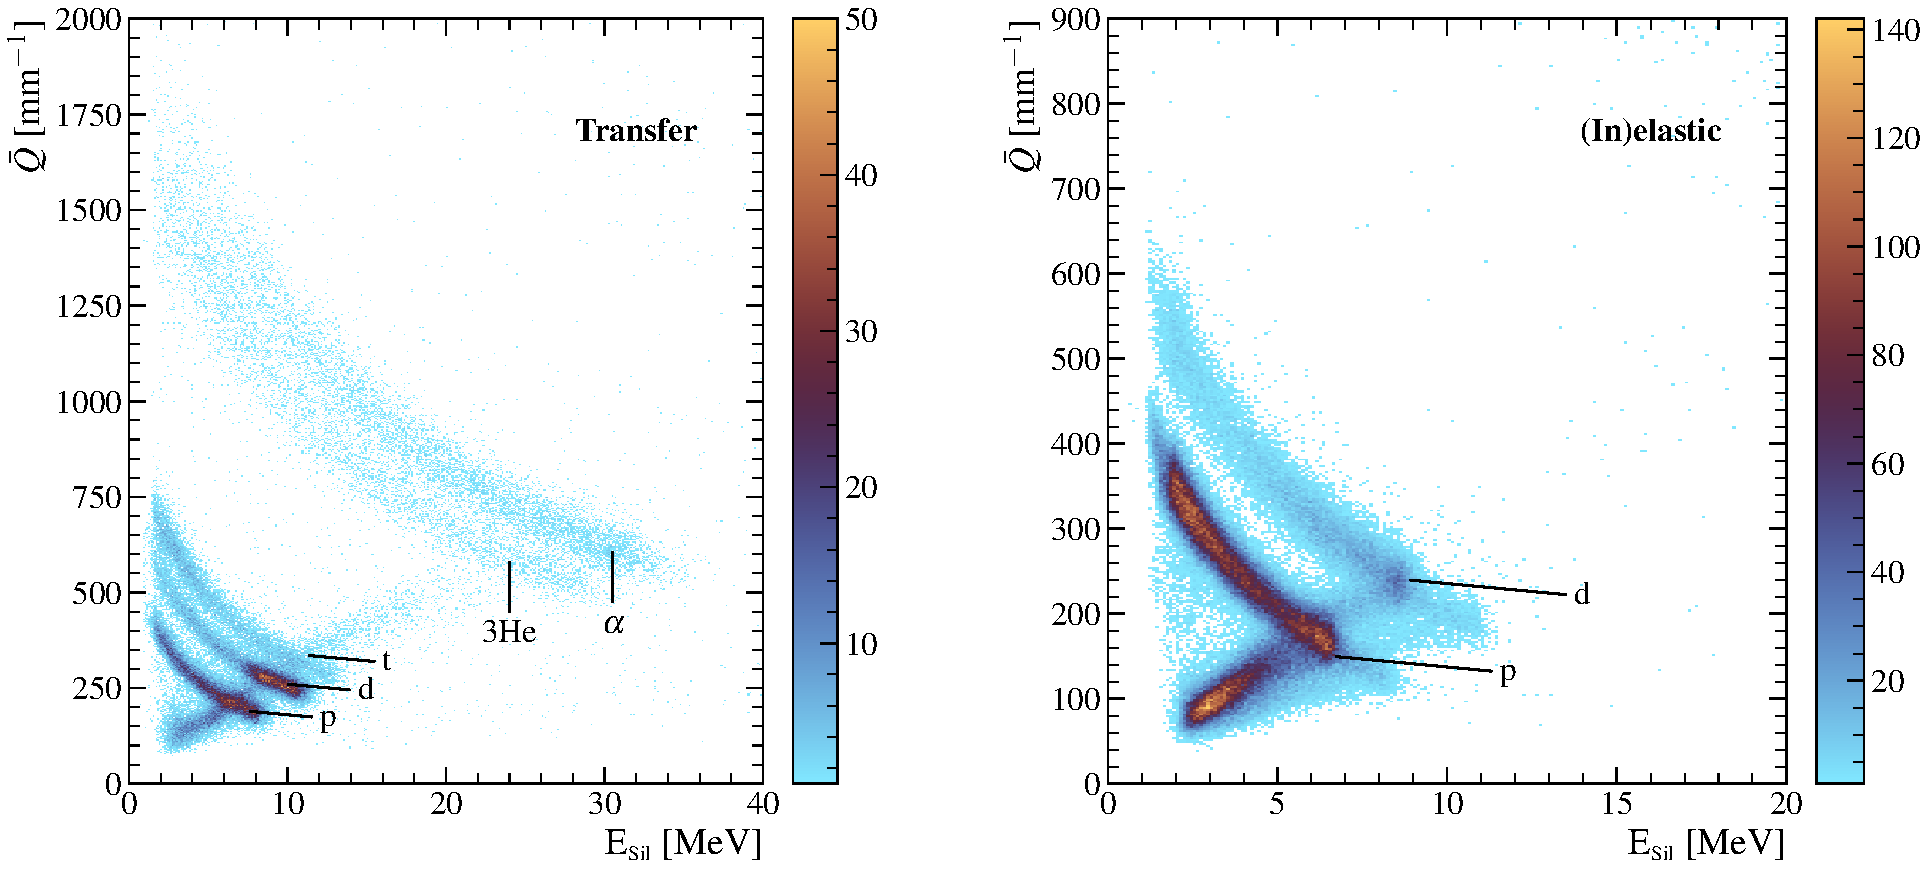
\includegraphics[width=0.95\textwidth]{figures/pid.pdf}
	\end{figure}
	\begin{columns}[c]
		\begin{column}{0.5\linewidth}
			\mycolorbox[1]{boxPink}{
				Good PID after vetoing punchthrough
			}
		\end{column}% 
		\begin{column}{0.5\linewidth}
			\mycolorbox[1]{boxGreen}{
				Only p and d for side silicons
			}
		\end{column}
	\end{columns}



\end{frame}

\section{Results}
\begin{frame}{Results: (in)elastic scattering}
	These are the excitation energy spectra for protons and deuterons.
	\begin{figure}
		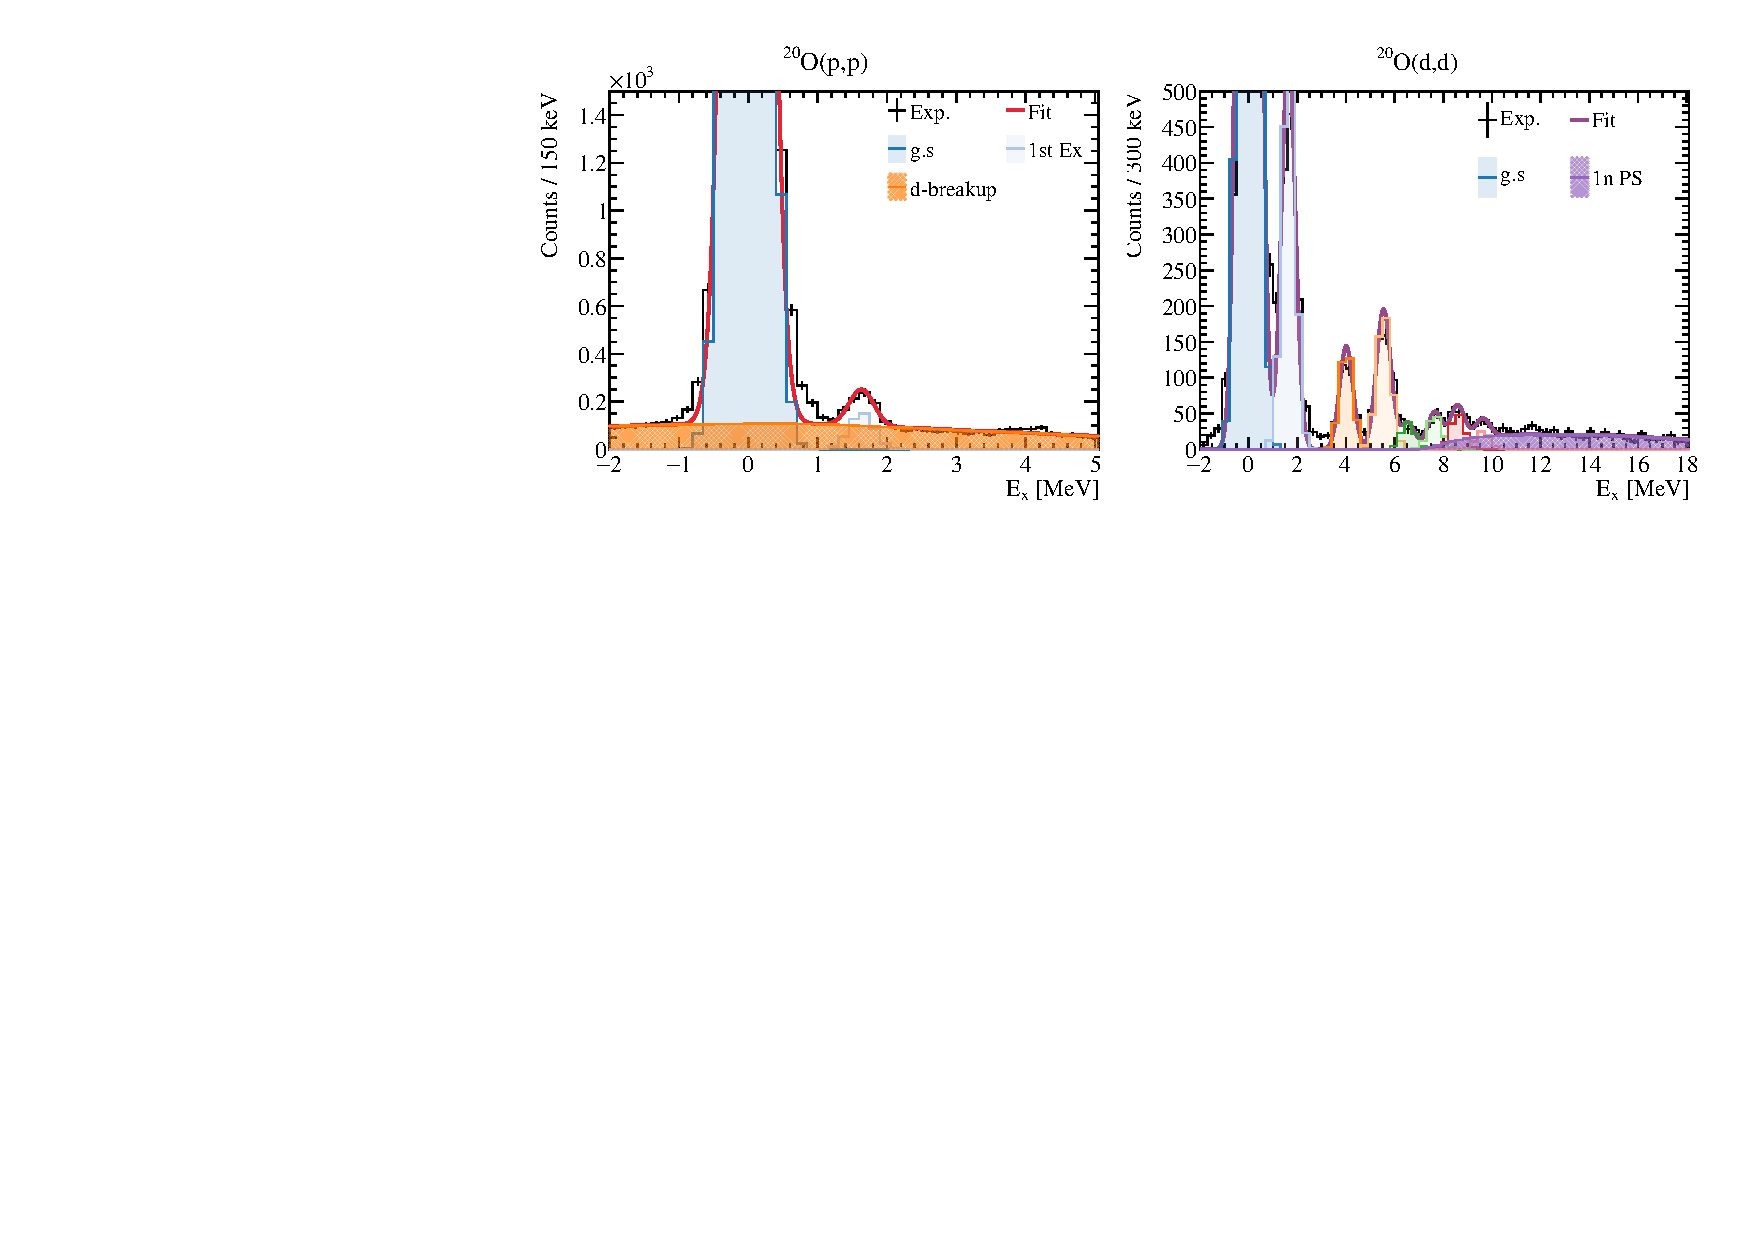
\includegraphics[width=0.95\textwidth]{figures/elastic_xs.pdf}
		% \caption{}
	\end{figure}
	\begin{columns}[c]
		\begin{column}{0.45\linewidth}
			\mycolorbox{box1}{Only 1st excited state}
		\end{column}%
		\begin{column}{0.45\linewidth}
			\mycolorbox{box2}{
				Up to 7 $E_{x} > 0$ states observed!
			}
		\end{column}
	\end{columns}
\end{frame}

\begin{frame}{Results: \iso{20}{O}(d,d)}
	Angular distributions for the \textbf{ground state} and first excited states:
	\begin{figure}
		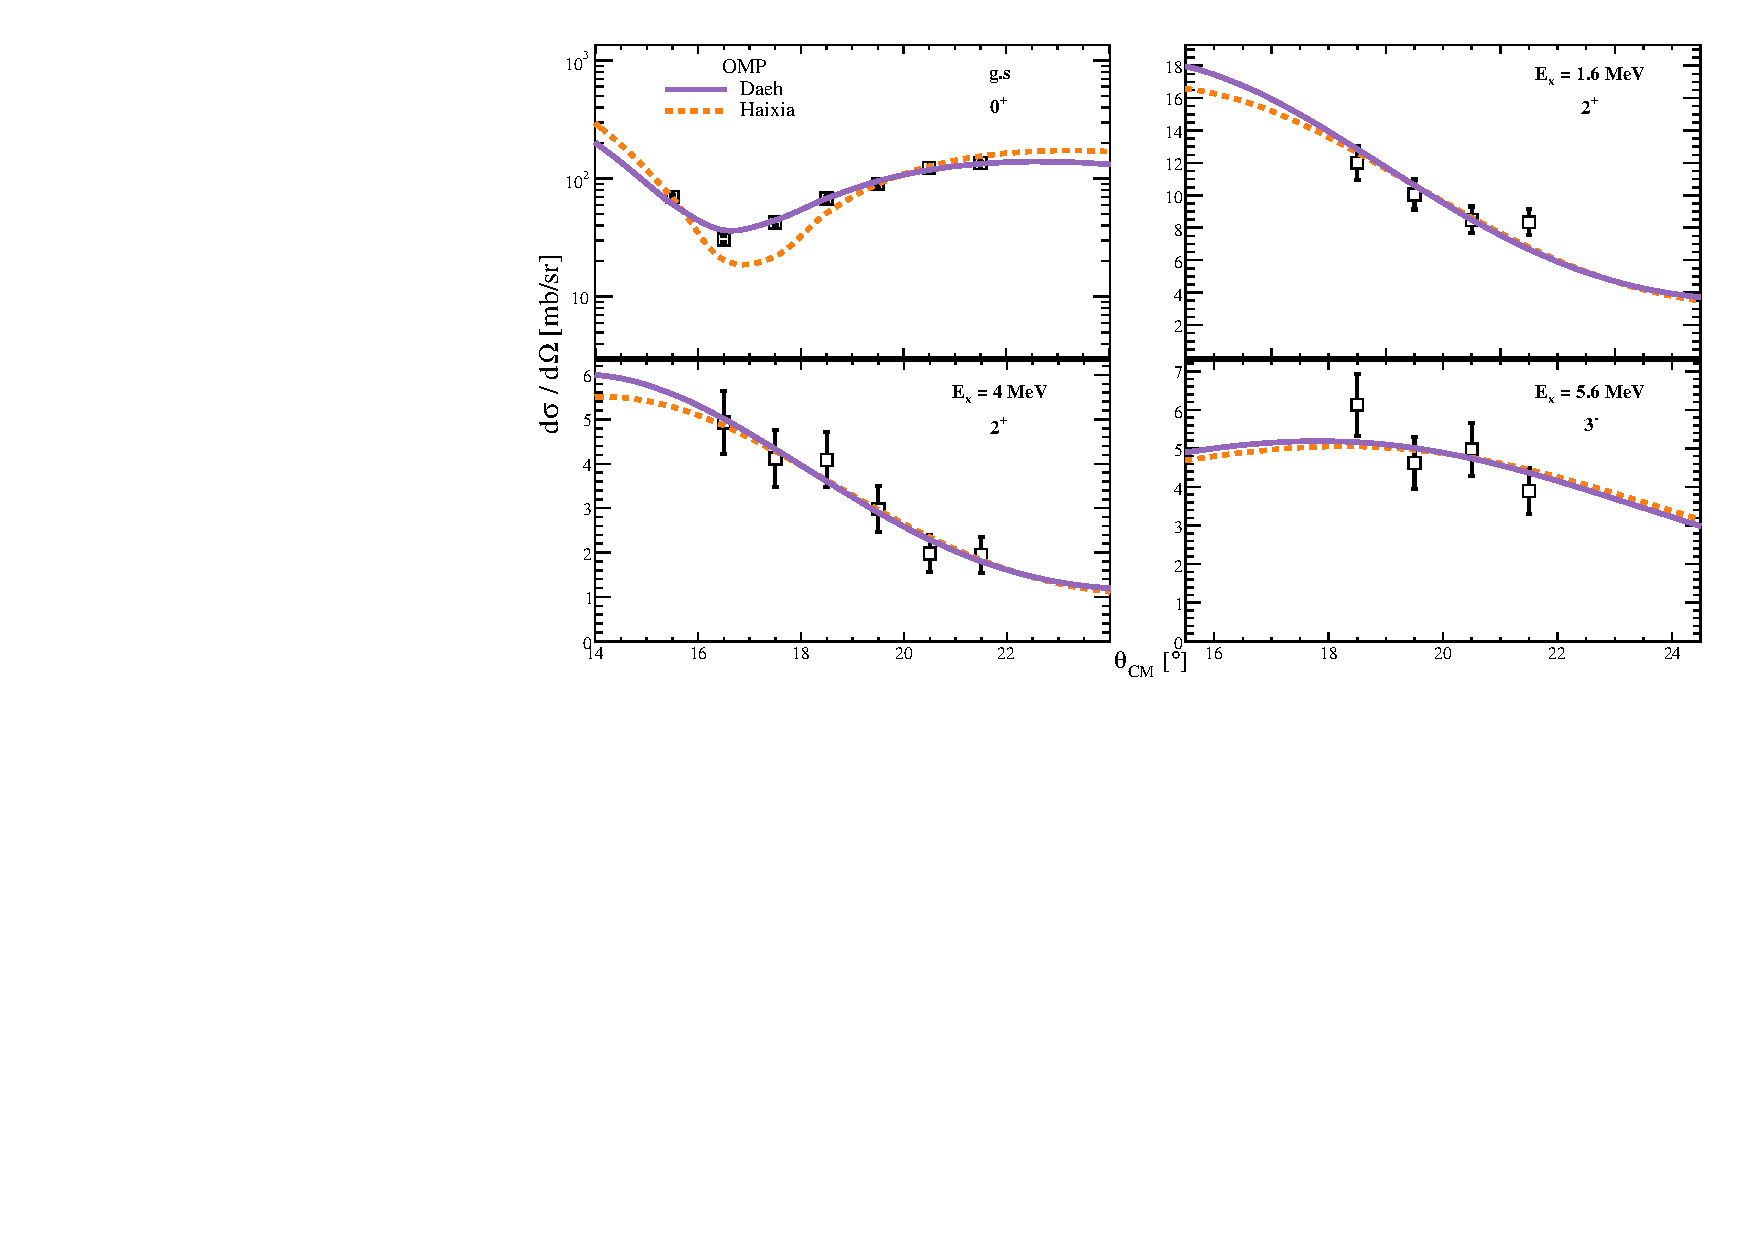
\includegraphics[width=0.85\linewidth]{figures/d_ang.pdf}
	\end{figure}
	\mycolorbox{box3}{Remaining states: low stats. Coming soon.}
\end{frame}

\begin{frame}{Results: \iso{20}{O}(p,p)}
	For the proton scattering:
	\begin{figure}
		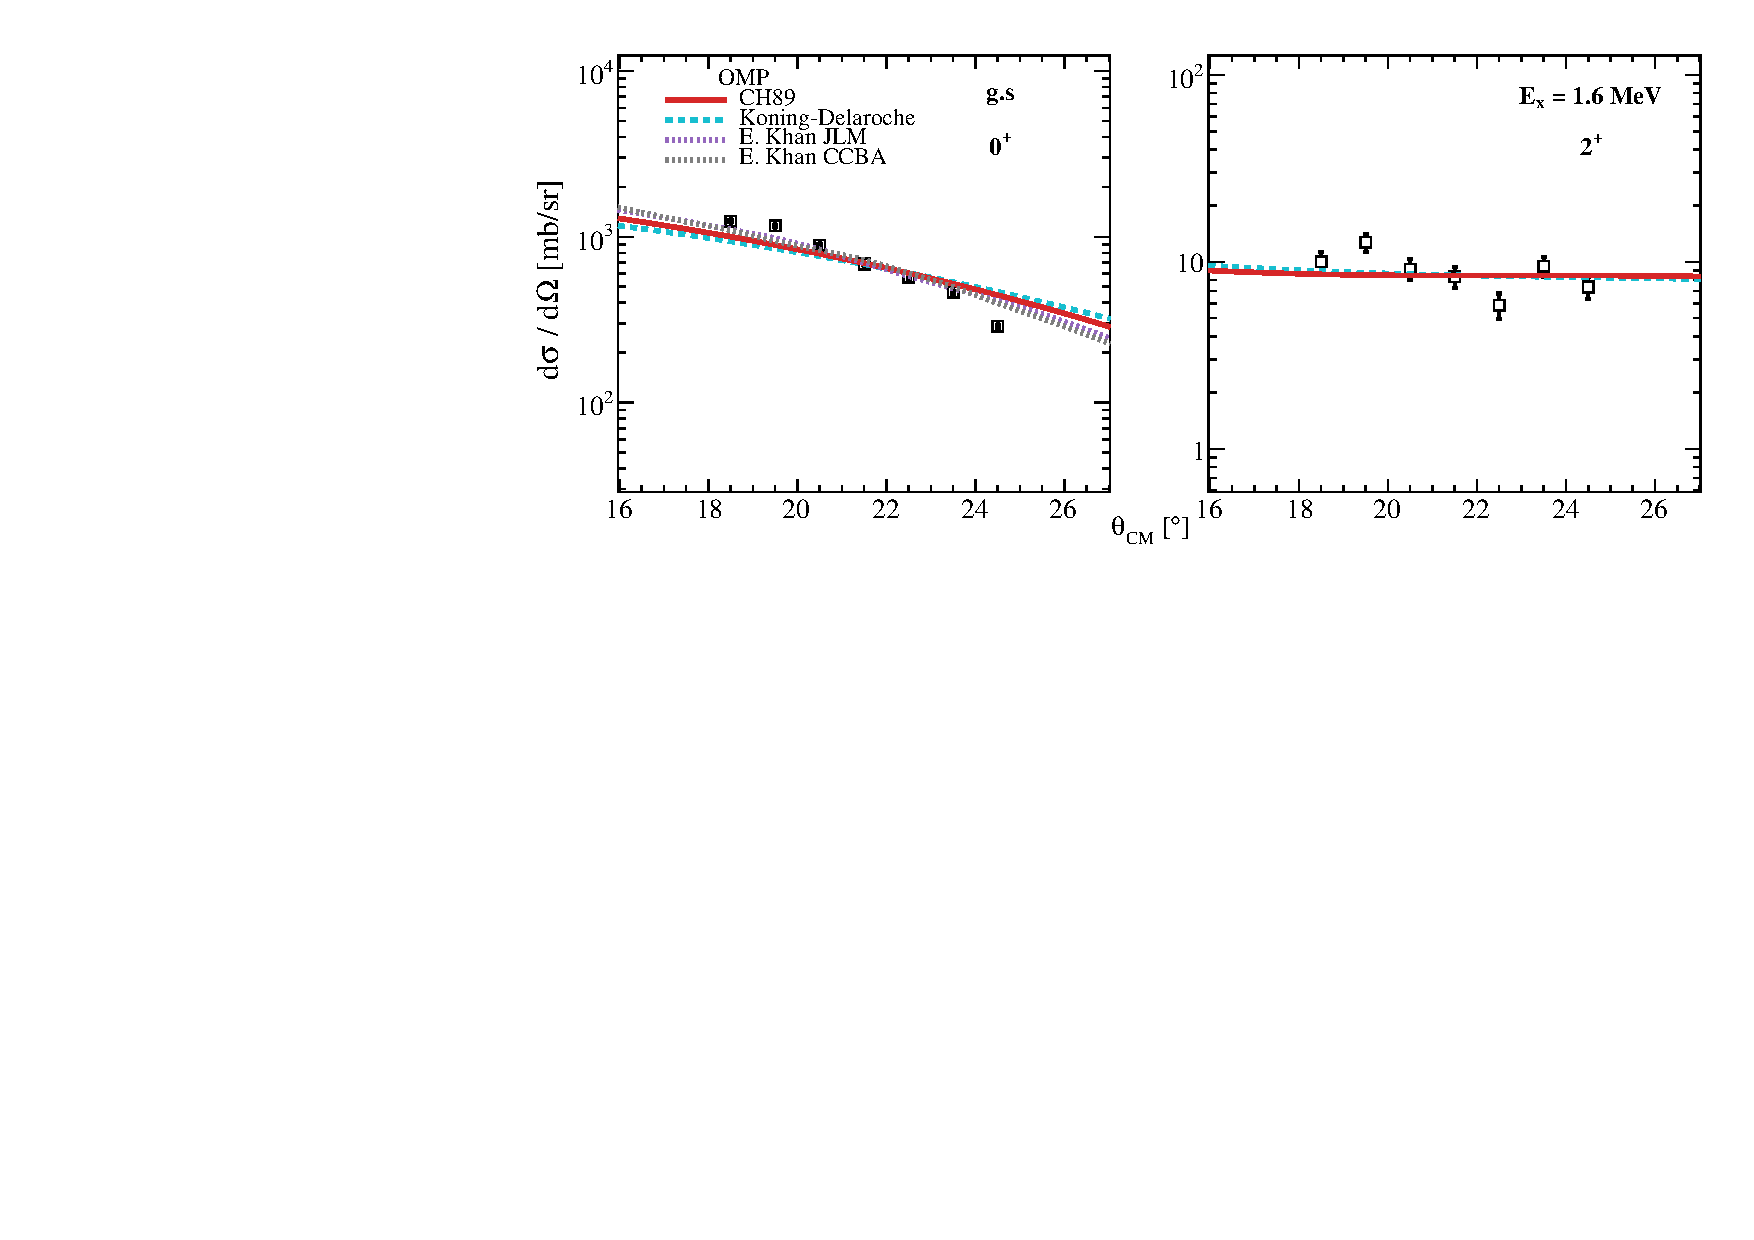
\includegraphics[width=0.85\textwidth]{figures/p_ang.pdf}
	\end{figure}
	\begin{columns}[c]
		\begin{column}{0.55\linewidth}
			\mycolorbox{box2}{
				\textbf{Issue}: gs not reproduced by any OMP!\\
				\emoji{cold-sweat}
			}
		\end{column}%
		\begin{column}{0.45\linewidth}
			\mycolorbox[0.9]{box4}{
				1st excited seems fine
			}
		\end{column}
	\end{columns}

\end{frame}

\begin{frame}{About normalizations}
	Just to recall the xs formula:
	\begin{equation*}
		\frac{d\sigma}{d\Omega} = \frac{N}{ \textcolor{red}{N_{\text{beam}}N_{\text{targets}}} \epsilon \Delta \Omega} = \frac{N}{ \textcolor{red}{\alpha} \epsilon \Delta \Omega}
	\end{equation*}
	\begin{columns}[c]
		\begin{column}{0.5\linewidth}
			\mycolorbox[1]{box2}{
				\begin{itemize}
					\item $N_{\text{beam}} \leftarrow$ CFA counter
					\item $N_{\text{targets}} \leftarrow$ Gas mixture. Sensitive to p.
				\end{itemize}
				Theo. lines need \textbf{scaling} ($\alpha$) to match experimental data\\
				$\alpha$ in agreement with Juan's\\
				$\Rightarrow$ Not likely $\epsilon$ issue
				% 	% Not likely an issue of reconstruction $\epsilon$
			}
		\end{column}%
		\begin{column}{0.5\linewidth}
			\mycolorbox[1]{box4}{
				Which norm should we use?
				\begin{figure}
					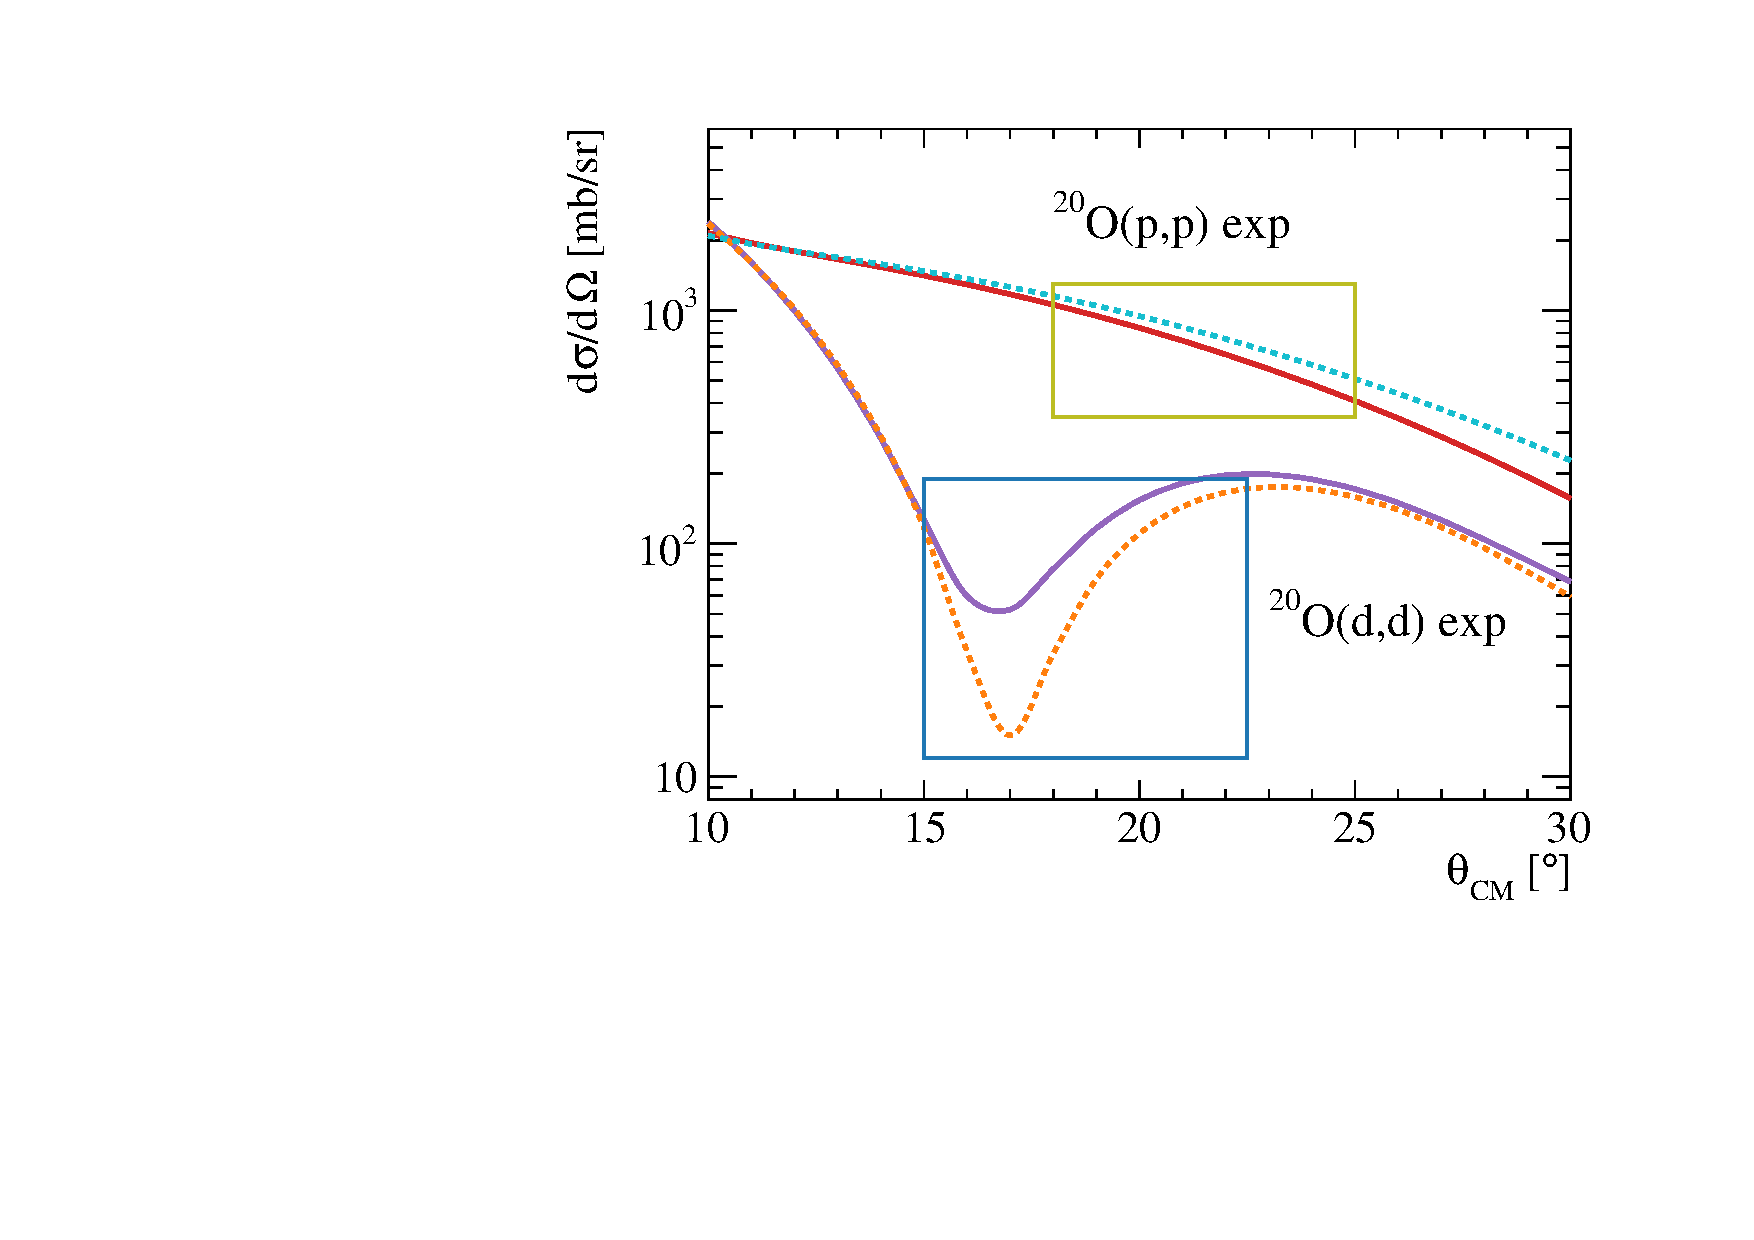
\includegraphics[width=0.9\textwidth]{figures/theo.pdf}
				\end{figure}
				Protons are more "reliable" \emoji{thinking}
			}
		\end{column}
	\end{columns}
\end{frame}

\begin{frame}{Results: \iso{20}{O}(d,t)}
	Excited states are populated up to $\sim\qty{15}{\MeV}$:
	\begin{figure}
		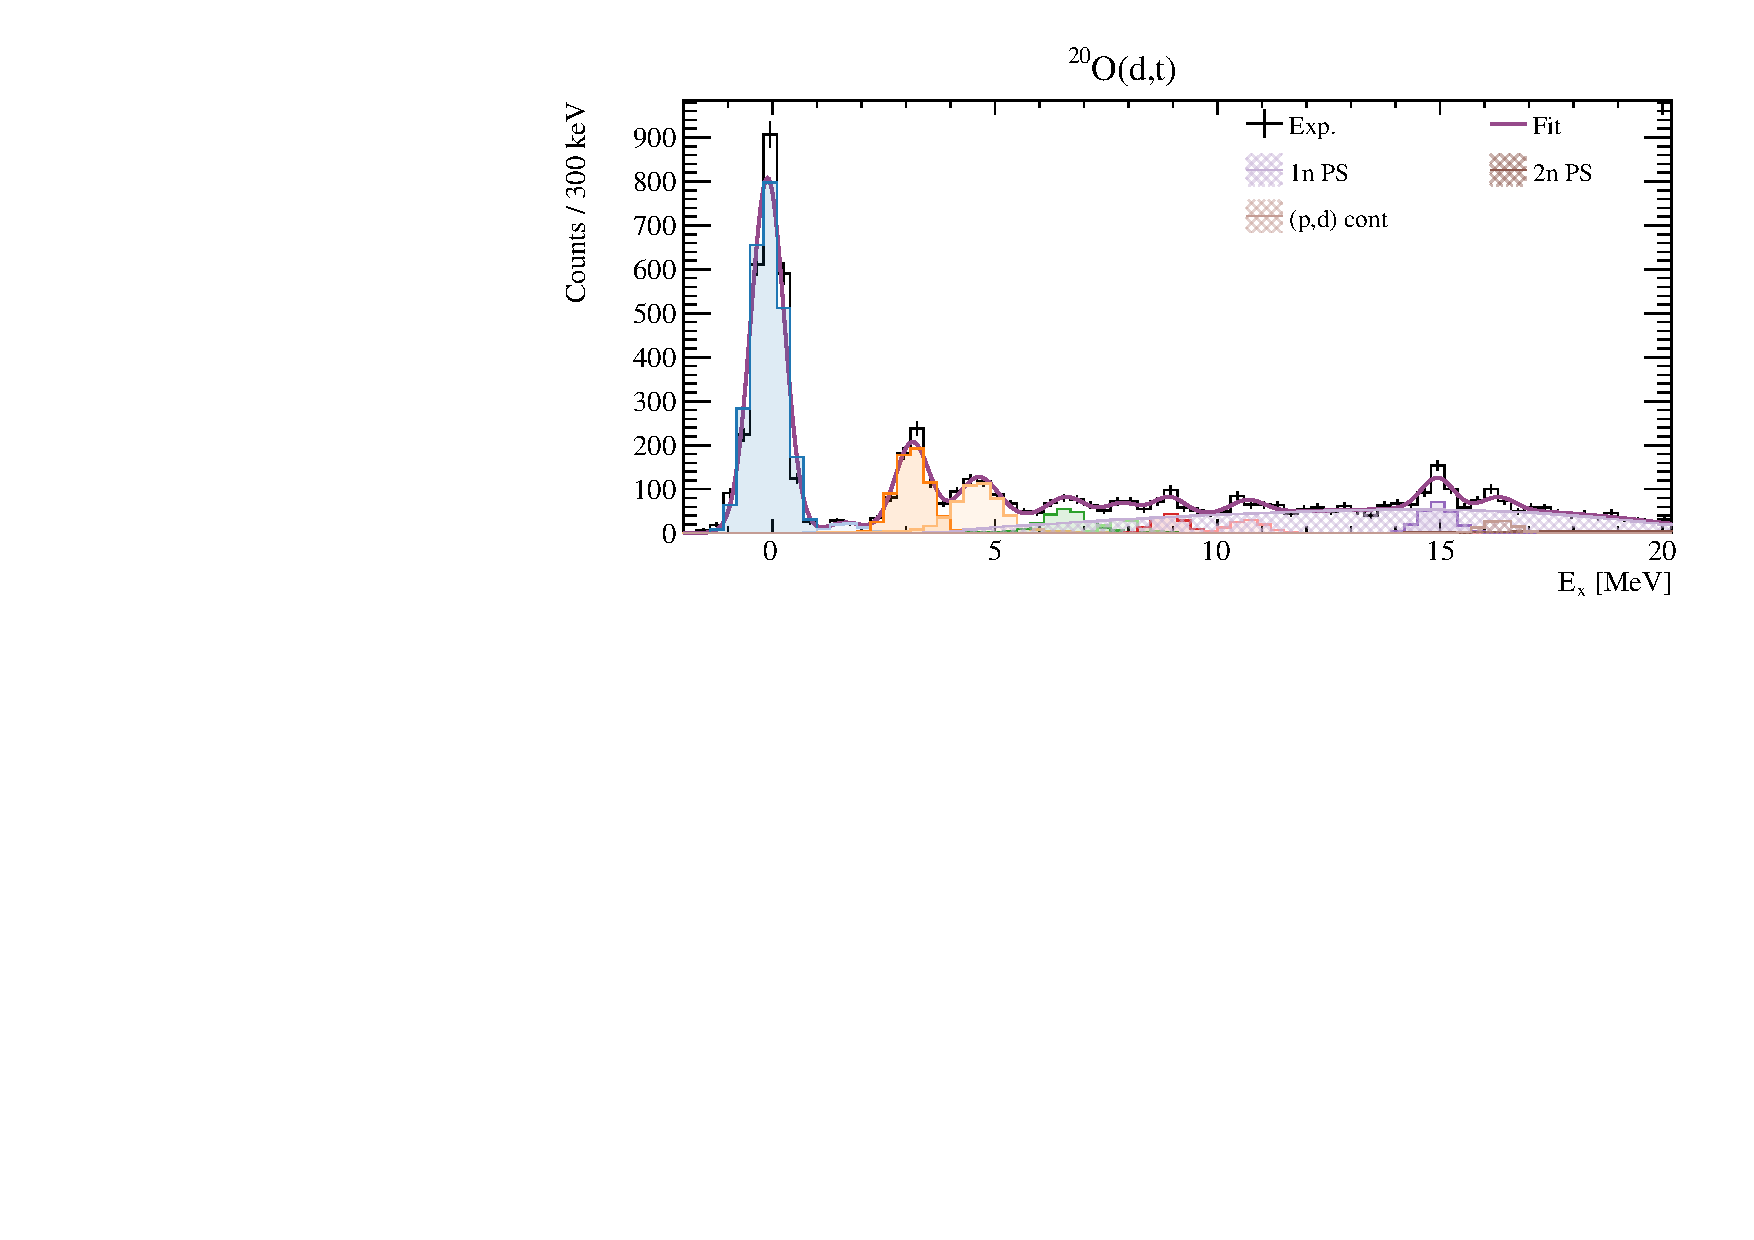
\includegraphics[width=0.95\textwidth]{figures/dt_xs.pdf}
	\end{figure}
	\mycolorbox{box3}{
		1n and 2n \textbf{phase spaces} are included in the fit. Small (p,d) contamination at $\sim \qty{16}{\MeV}$ under control.
	}
\end{frame}

\begin{frame}{Results: \iso{20}{O}(d,t)}
	Fresco DWBA with OMPs: Daehnick (d), Pang (t)
	\only<+>{
		\begin{figure}
			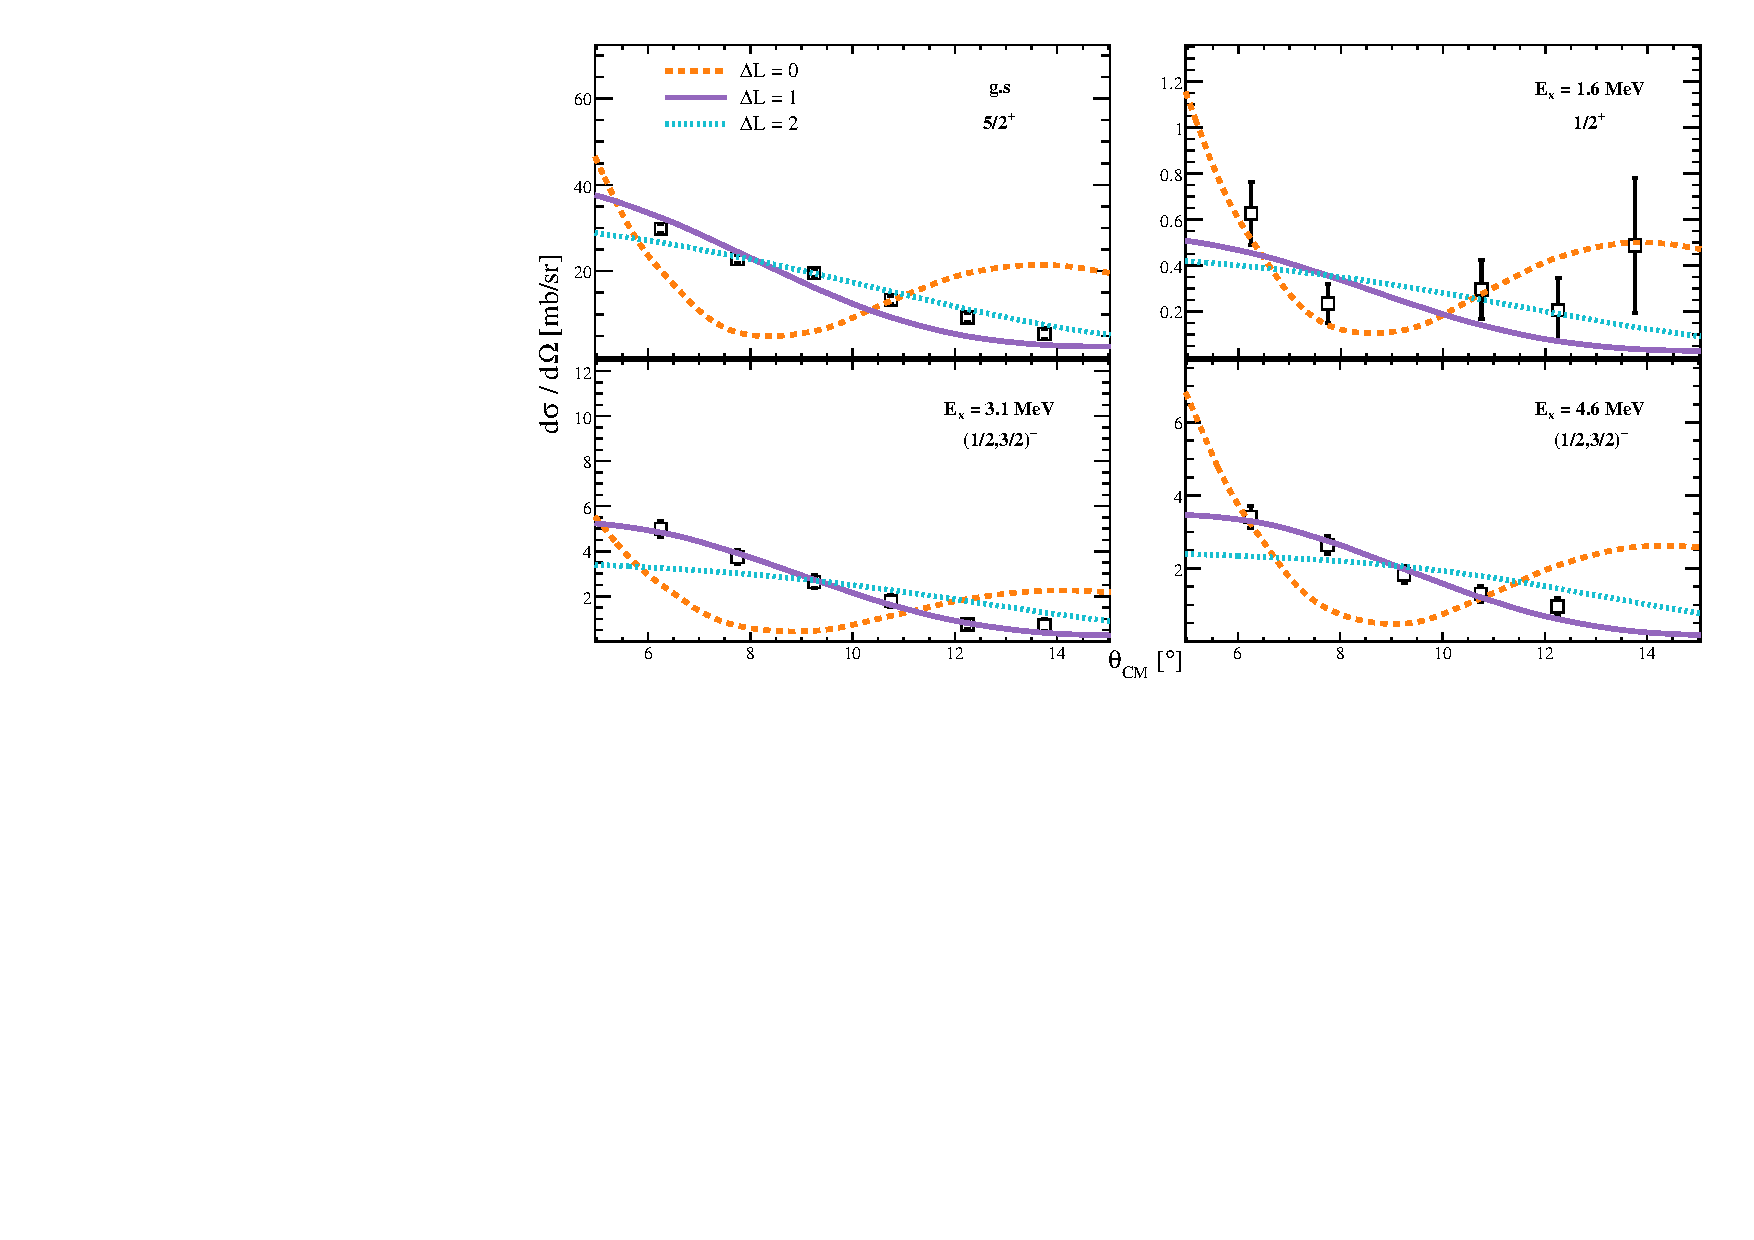
\includegraphics[width=0.95\textwidth]{figures/ang_0.pdf}
		\end{figure}
		\mycolorbox{box1}{
			Agreement with already known assignments.
		}
	}%
	\only<+>{
		\begin{columns}[c]
			\begin{column}{0.6\linewidth}
				\begin{figure}
					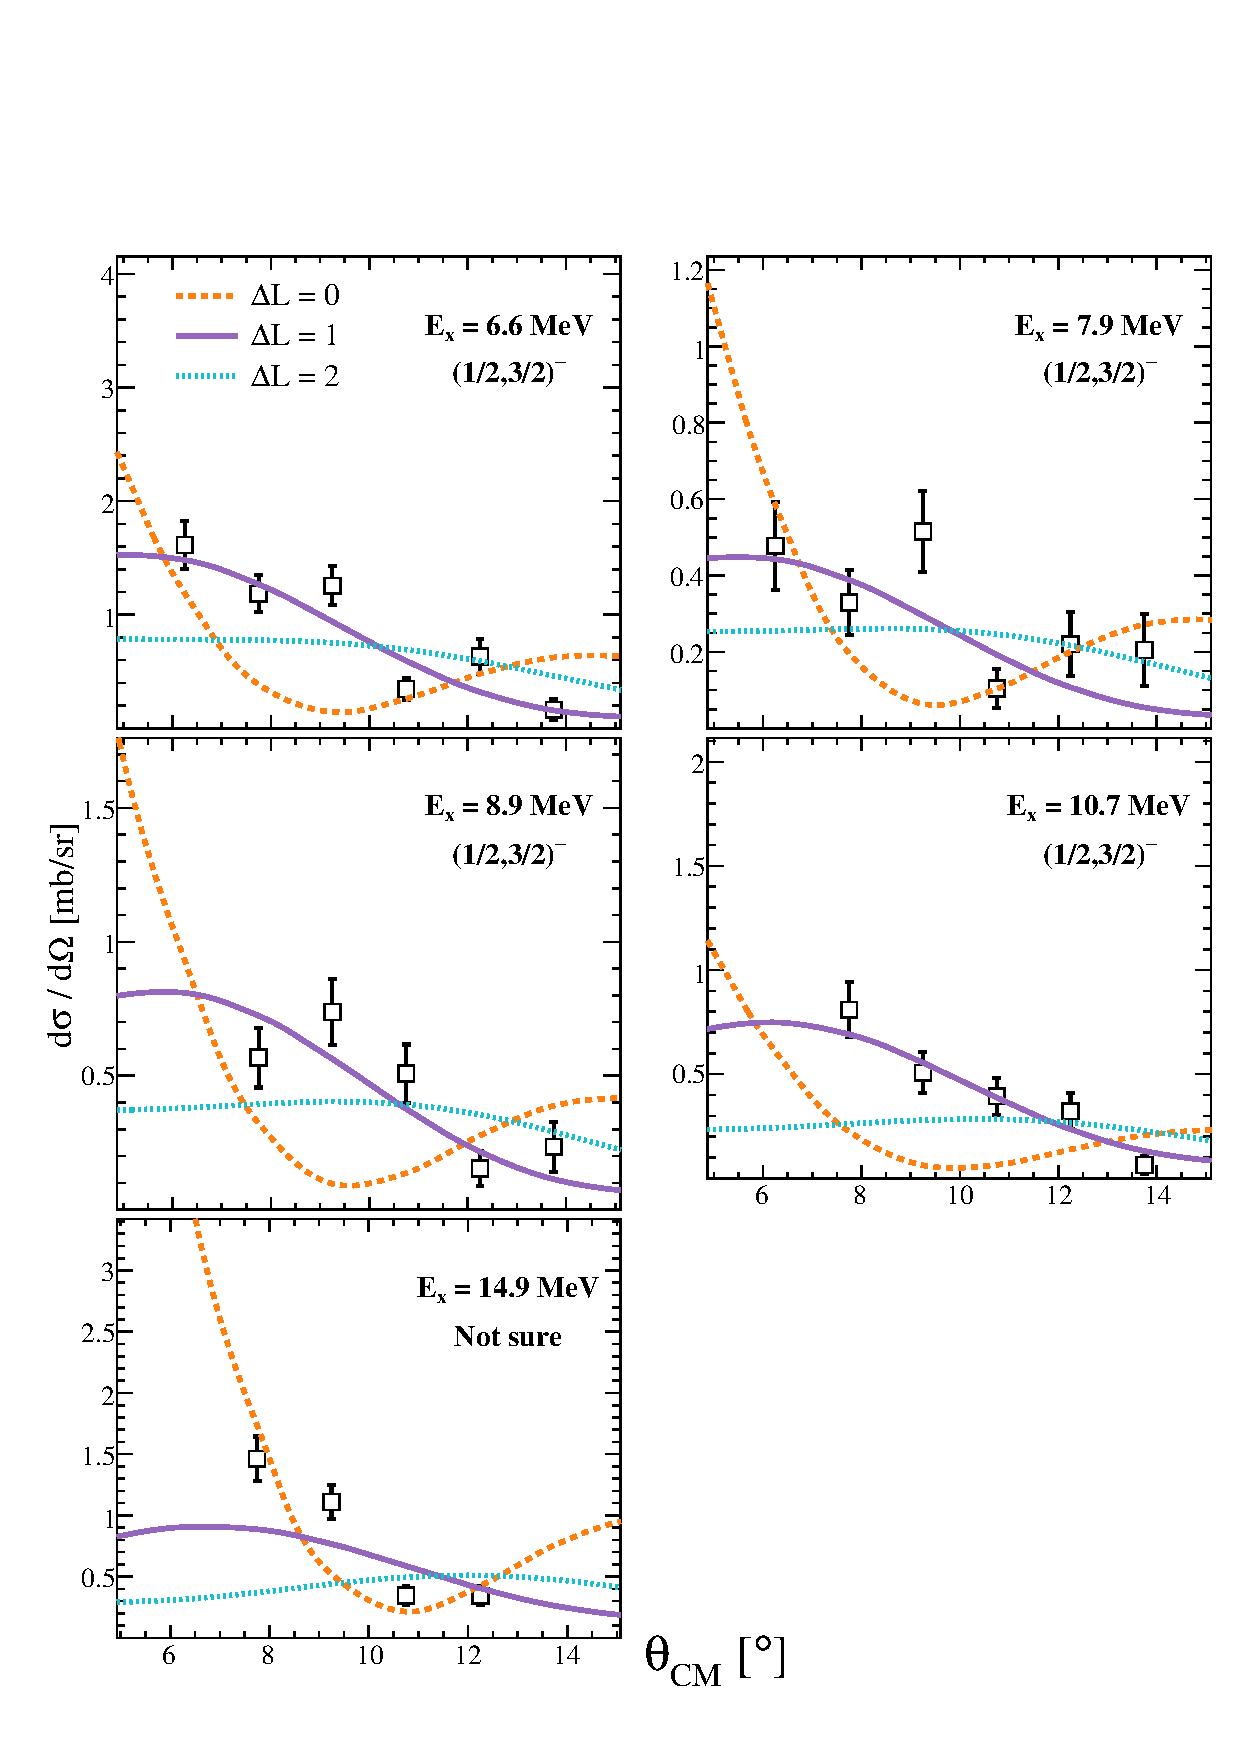
\includegraphics[height=0.75\textheight]{figures/ang_1.pdf}
				\end{figure}

			\end{column}%
			\begin{column}{0.4\linewidth}
				\mycolorbox{box3}{
					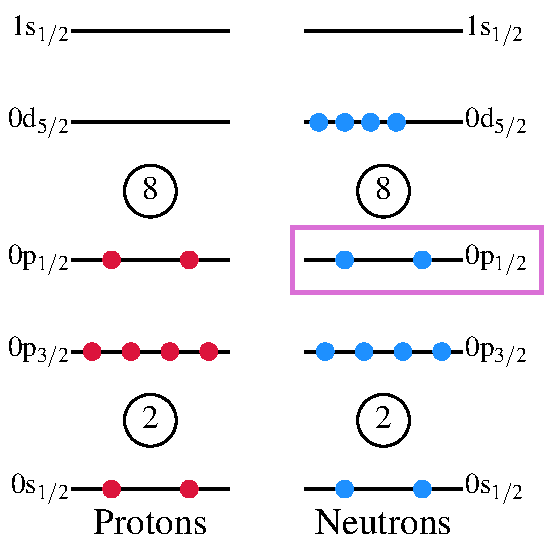
\includegraphics[width=0.9\linewidth]{figures/sm_l1.pdf}
					% Few stats for some. Rebinning is foreseen.
				}\\
				\mycolorbox{boxPink}{
					Almost all are $\Delta L = 1$!
				}\\ 
        \mycolorbox{boxBrown}{
          SFO-tls and YSOX $\Rightarrow 0p_{1/2}$
        }
			\end{column}
		\end{columns}
	}
\end{frame}

% \begin{frame}{Results: \iso{20}{O}(d,t)}
% 	SF are compared with shell-model calculations with \textbf{YSOX} and \textbf{SFO-tls}.
% 	\begin{figure}
% 		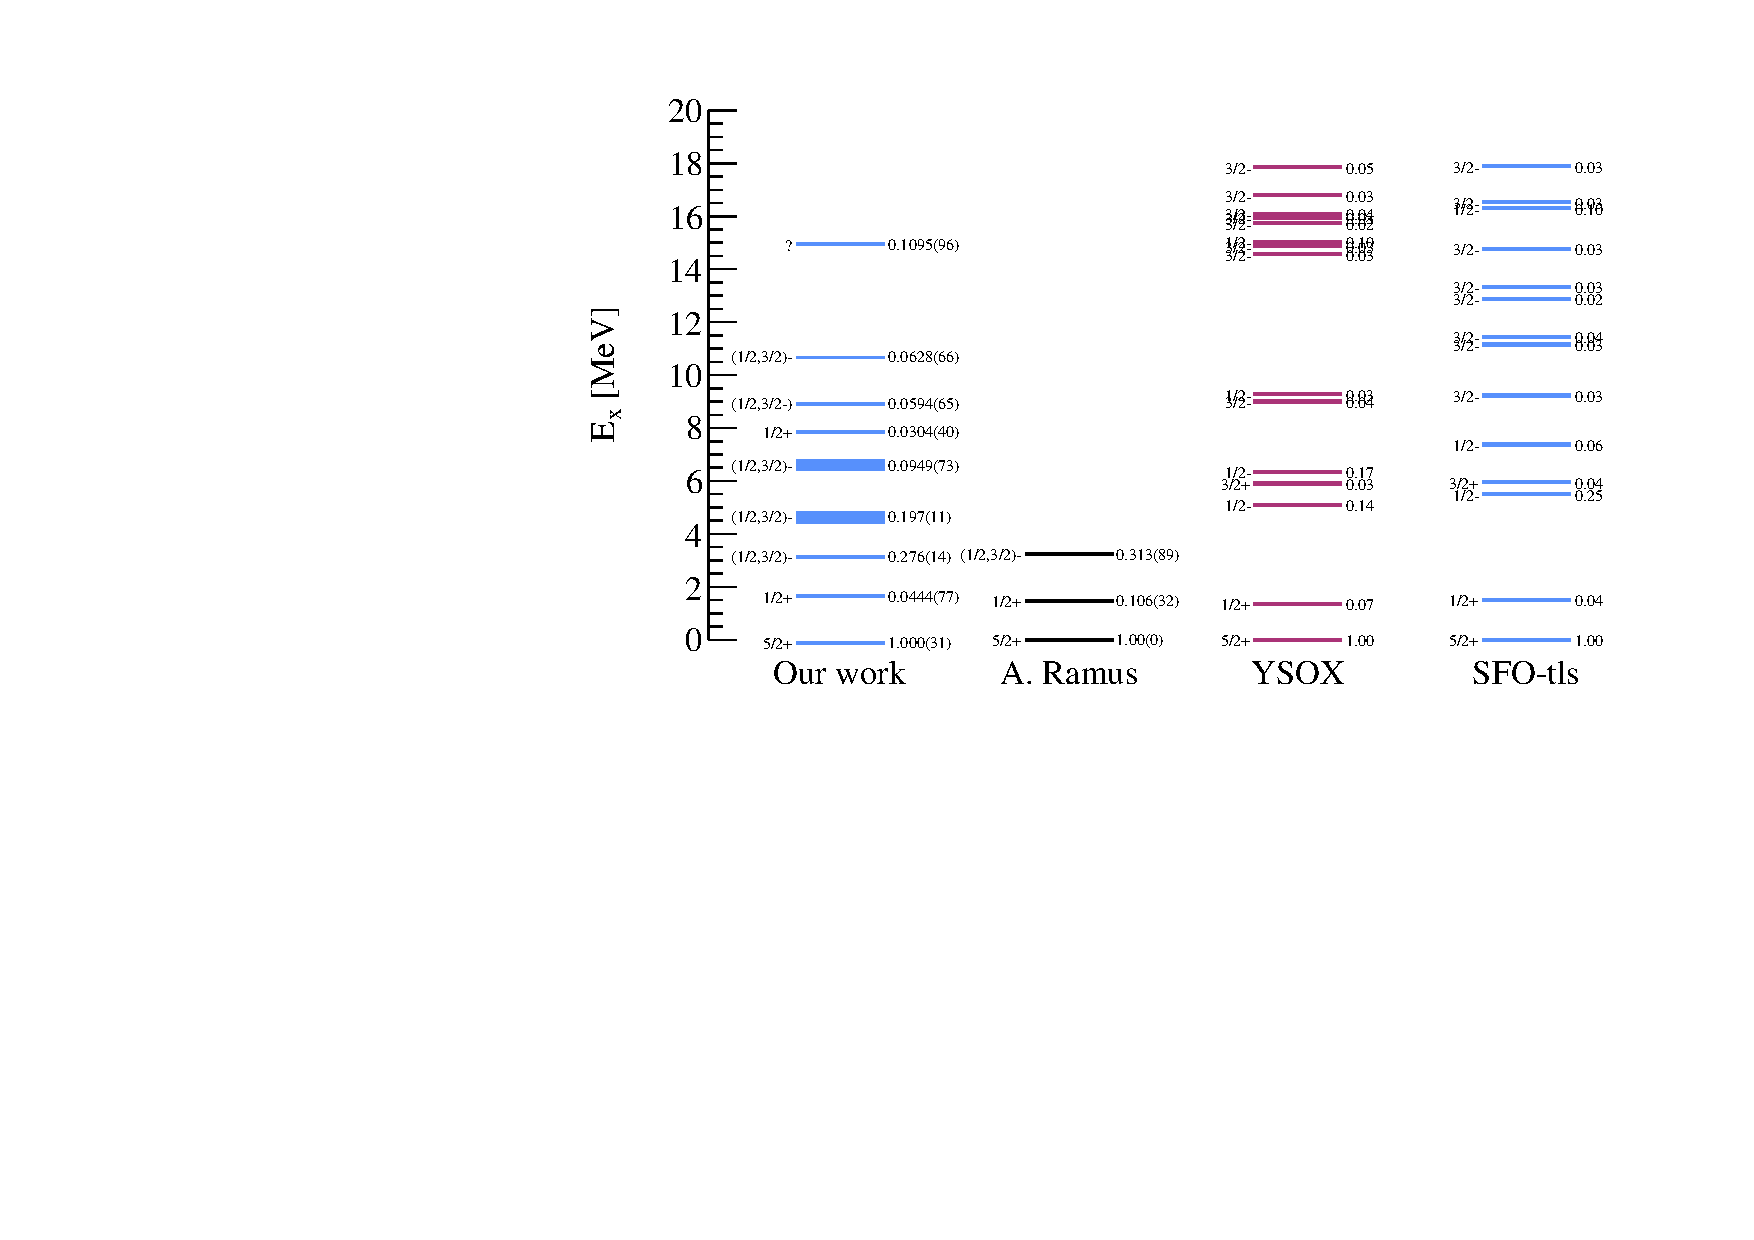
\includegraphics[width=0.8\textwidth]{figures/normalized_models.pdf}
% 	\end{figure}
% 	\begin{columns}[c]
% 		\begin{column}{0.5\linewidth}
% 			\mycolorbox[1]{box1}{
% 				\textbf{Normalized} to gs SF
% 			}
% 		\end{column}%
% 		\begin{column}{0.5\linewidth}
% 			\mycolorbox[1]{box2}{
% 				More $p_{1/2}$ strength than predicted at $E_{x} < \qty{10}{\MeV}$}
% 		\end{column}
% 	\end{columns}
% \end{frame}

\begin{frame}{About ESPEs}
	Effective single-particle energies (ESPEs) are needed to locate the $0p_{1/2}$ and $0d_{5/2}$ orbits: \textbf{Baranger's formula}
	\begin{equation*}
		\text{ESPE}_{nlj} = \frac{\sum_{i+}(2j + 1)\text{SF}_{i+}(E_{i+} - E_0) + \sum_{i-}\text{SF}_{i-}(E_{0} - E_{i-})}{\sum_{i+}(2j + 1)\text{SF}_{i+} + \sum_{i-}\text{SF}_{i-}}
	\end{equation*}
	\begin{columns}[c]
		\begin{column}{0.5\linewidth}
			\mycolorbox{box1}{
				\textbf{Removal} ($-$) from our (d,t) or (p,d) channels.
			}
		\end{column}%
		\begin{column}{0.5\linewidth}
			\mycolorbox{box2}{
			\textbf{Adding} ($+$) from \iso{20}{O}(d,p)\iso{21}{O} by\\
			{\small B. Fernández-Domínguez \textit{et al.} PRC 84 (2011)}
			}
		\end{column}
	\end{columns}
\end{frame}

\begin{frame}{Results: \iso{20}{O}(d,t)}
	All $\Delta L = 1$ states below $E_{x} = \qty{10}{\MeV}$ are $p_{1/2}$ based on YSOX and SFO-tls
	\begin{figure}
		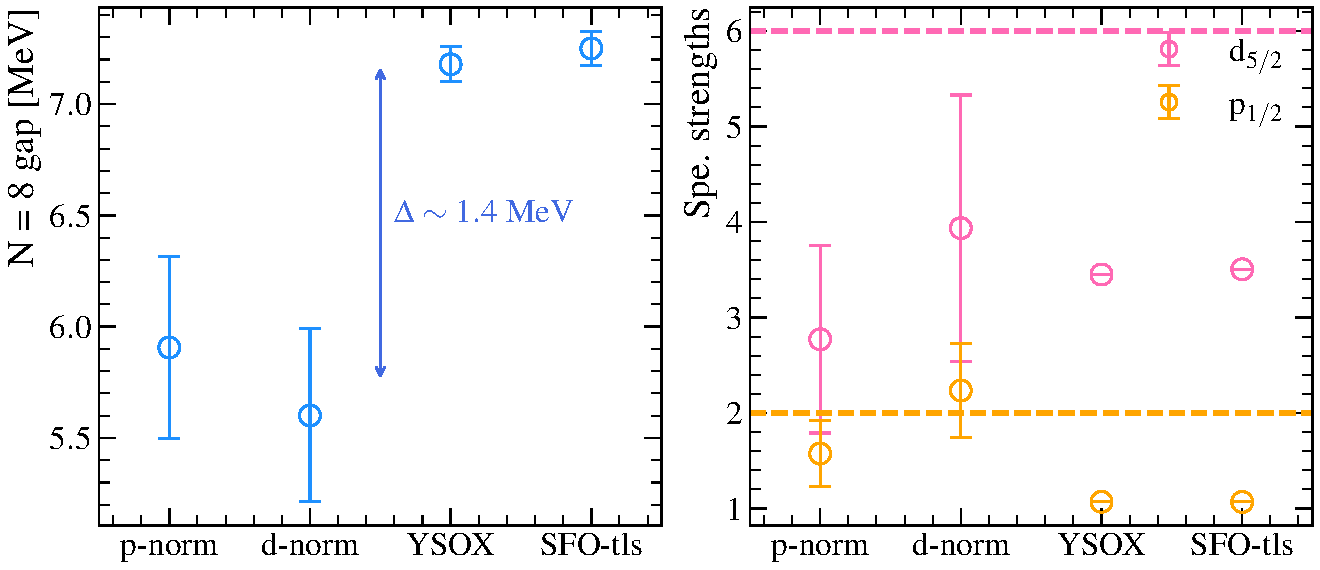
\includegraphics[width=0.75\textwidth]{figures/gap.pdf}
	\end{figure}
	\begin{columns}[c]
		\begin{column}{0.5\linewidth}
			\mycolorbox{box3}{
				\textbf{Smaller} experimental gap than predicted!
			}
		\end{column}%
		\begin{column}{0.5\linewidth}
			\mycolorbox{box2}{
				Higher $0p_{1/2}$ occupation according to exp.
			}
		\end{column}
	\end{columns}
	{\footnotesize Note: \textit{p-norm} refers to absolute SFs with (p,p) normalization, whereas \textit{d-norm} to (d,d) data}
\end{frame}

\begin{frame}{Results: \iso{20}{O}(p,d)}
	Fewer states are populated in this channel:
	\begin{figure}
		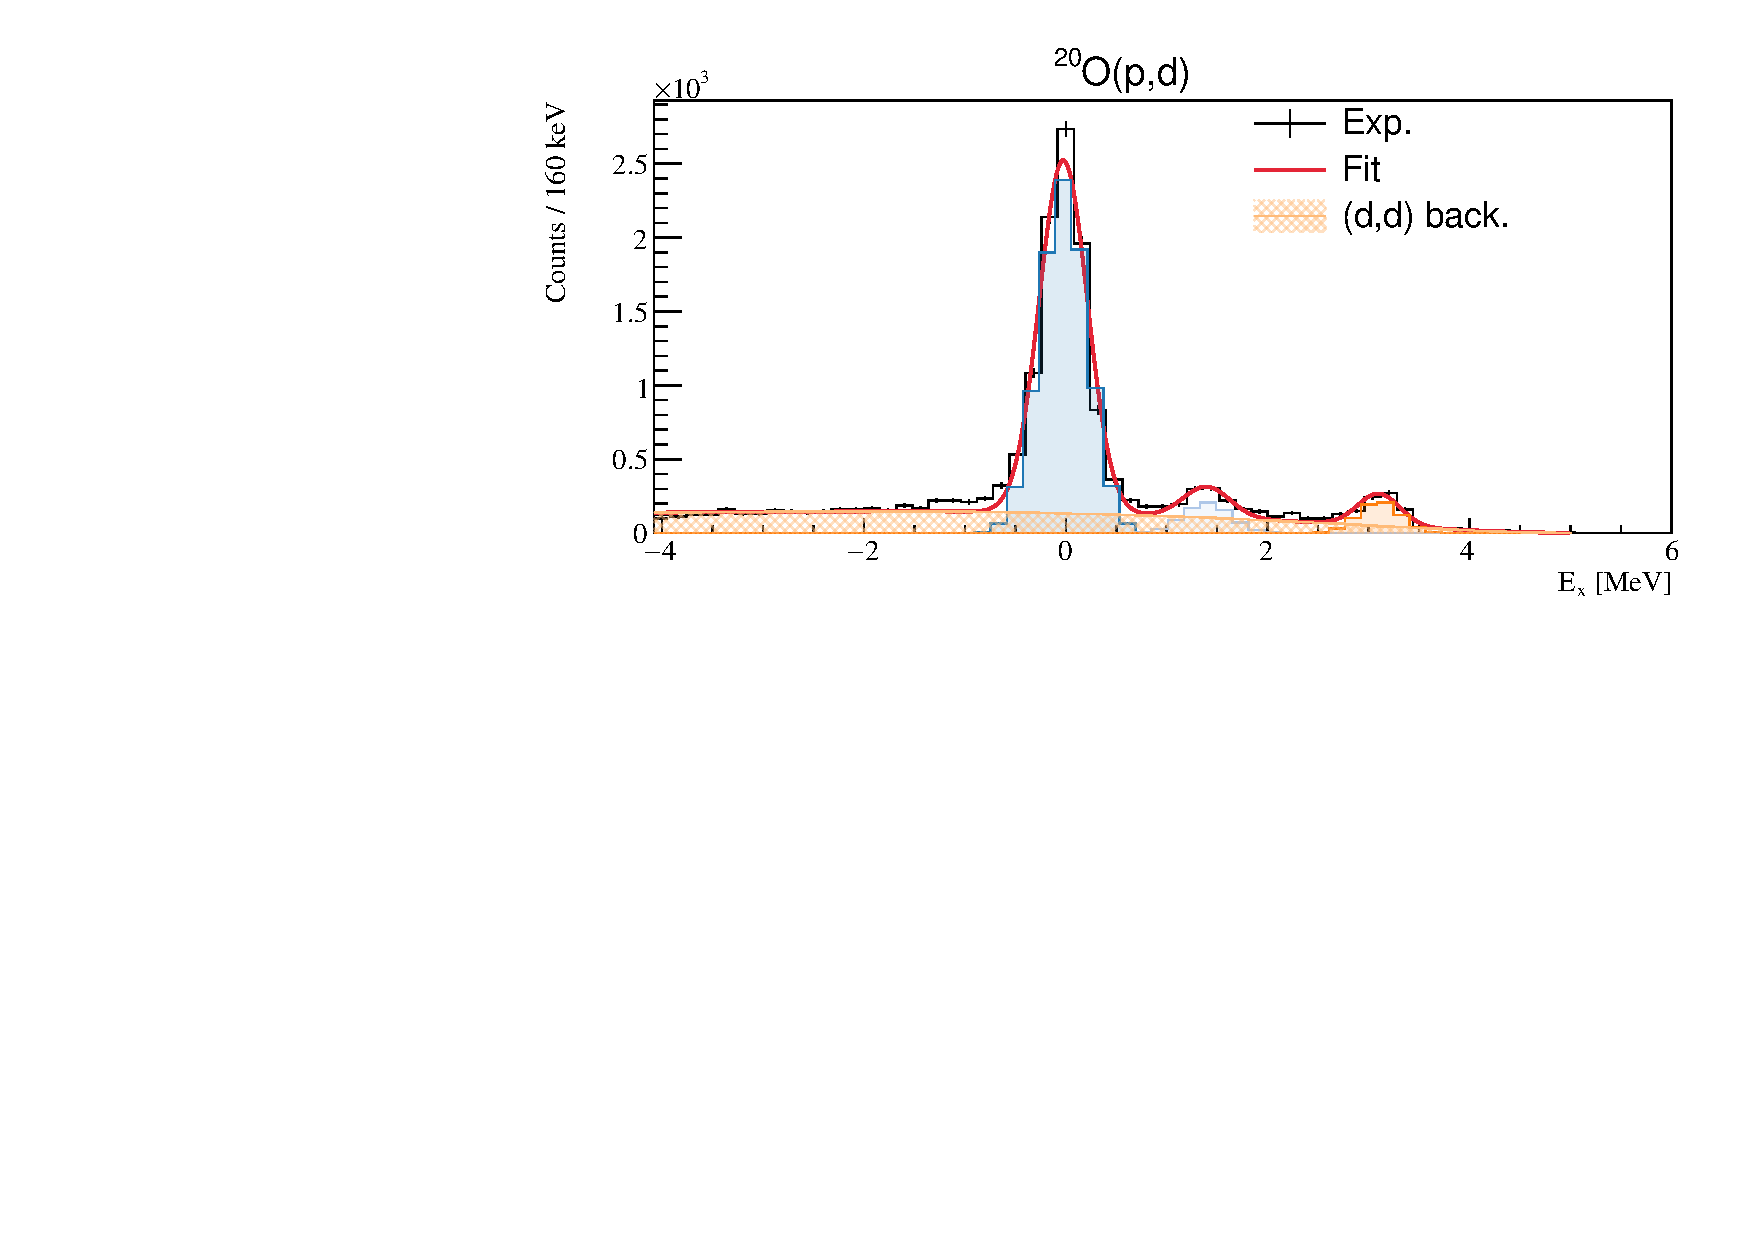
\includegraphics[width=0.95\textwidth]{figures/pd_xs.pdf}
	\end{figure}
	\mycolorbox{box2}{
		Strong (d,d) background since we only identify the outgoing deuteron!
	}

\end{frame}

\begin{frame}{Results: \iso{20}{O}(p,d)}
	OMPs: CH89 (p), ADWA (d). Not so encouraging results:
	\begin{figure}
		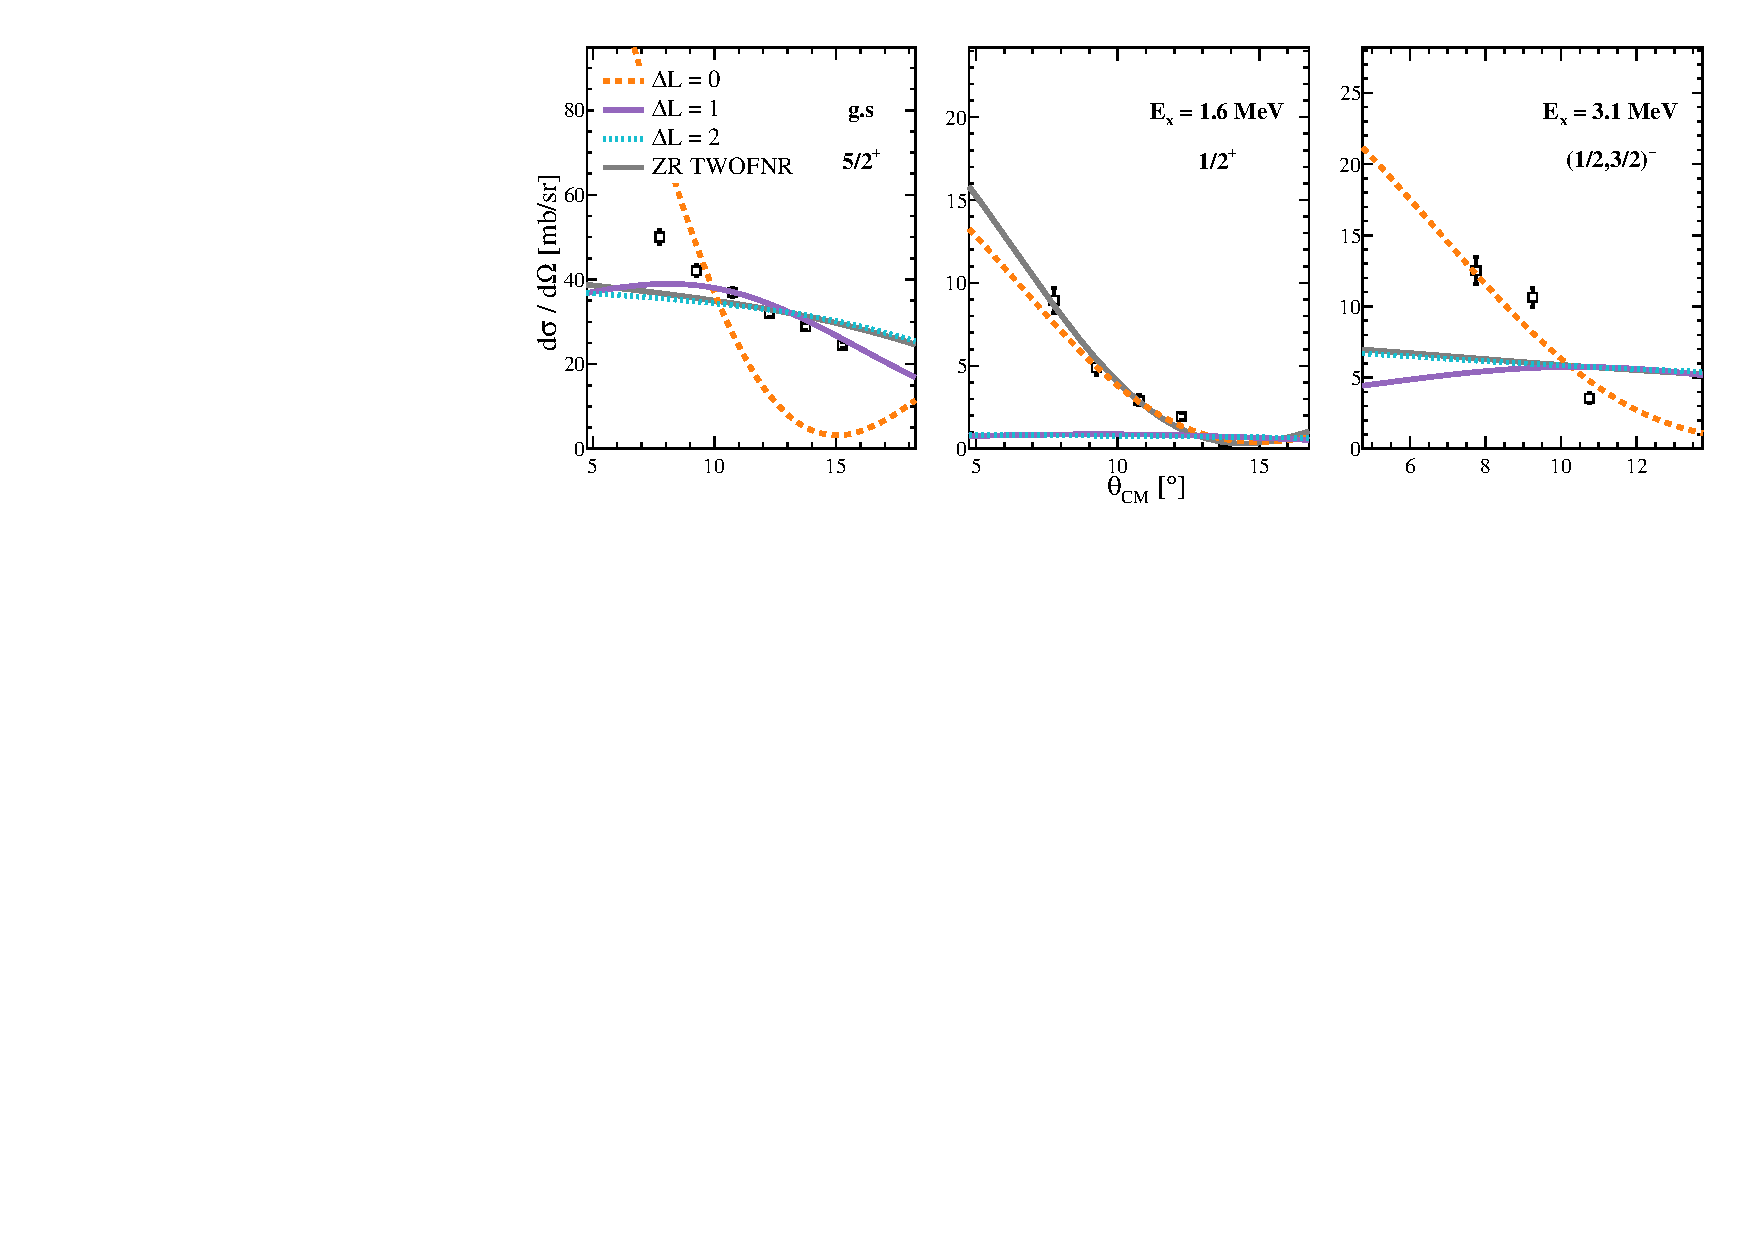
\includegraphics[width=0.95\textwidth]{figures/pd_ang_0.pdf}
	\end{figure}
	\begin{columns}[c]
		\begin{column}{0.5\linewidth}
			\mycolorbox{boxBrown}{
				Either Fresco or ZR Twofnr fail to reproduce \textbf{gs} \emoji{confused}
			}
		\end{column}%
		\begin{column}{0.5\linewidth}
			\mycolorbox{boxGreen}{
				Yet 1st excited state seems well-reproduced!
				\emoji{raised-eyebrow}
			}
		\end{column}
	\end{columns}
\end{frame}

\begin{frame}{Future work}
	\mycolorbox{box3}{
    Detailed study of \textbf{inelastic} channels
	}
	\vspace{1em}

	\mycolorbox{box2}{
    Solve normalization issue or find it an explanation
	}
	\vspace{1em}

	\mycolorbox{box4}{
    Ask theoreticians if interactions can be tuned for our data
	}
	\vspace{1em}

	\mycolorbox{box1}{
    Continue to investigate (p,p) and (p,d)
	}%
\end{frame}
\end{document}
